\documentclass[../Results.tex]{subfiles}
\begin{document}
	Fig. \ref{overlayspec} shows the HST image of MAMMOTH-1 with WFC F160W filter and contours for ly$\alpha$ HeII and CIV emission. All sources marked here are at z=2.3(confirmed by CO(1-0) emission from \cite{emonts2019cold} and Qiong (in prep)). It shows ly$\alpha$ emission extended $>20"$ which corresponds to $\approx170$kpc, this is the typical size of halo at this redshift. It covers all 8 sources here, this indicates that all of this sources could have contribution to illuminate this nebulae. We don't see this nebulae all because FoV of KCWI is $20" \times 16.8"$ and not that sensitive at the edges. Besides ly$\alpha$. Also we see HeII and CIV emission, contour shows signal beyond $3\sigma$ and $4\sigma$ for these two lines respectively. These two emissions are also extent because their size is larger than seeing and velocity gradient weighted from these 2 lines is significant (we would not see it if they are not resolved). The contour shows these two emission extended $> 6"$ which corresponds to physical projected scale of 50kpc. Besides, We don't find any significant HeII or CIV emission around other sources. 
	
	Fig. \ref{overlayspec} shows spectra extract in 1 $arcsec^{2}$ aperture centering on the flux peaks. We fit the three emission lines with single component gaussian function and also use the central wavelength fitted to calculate their redshifts, moreover we calculate their luminosity beyond $3\sigma$. We show these results and the fitting parameters in Tab. \ref{fit_L}. 
	\begin{figure*}
		\centering
		\subfloat[contour]{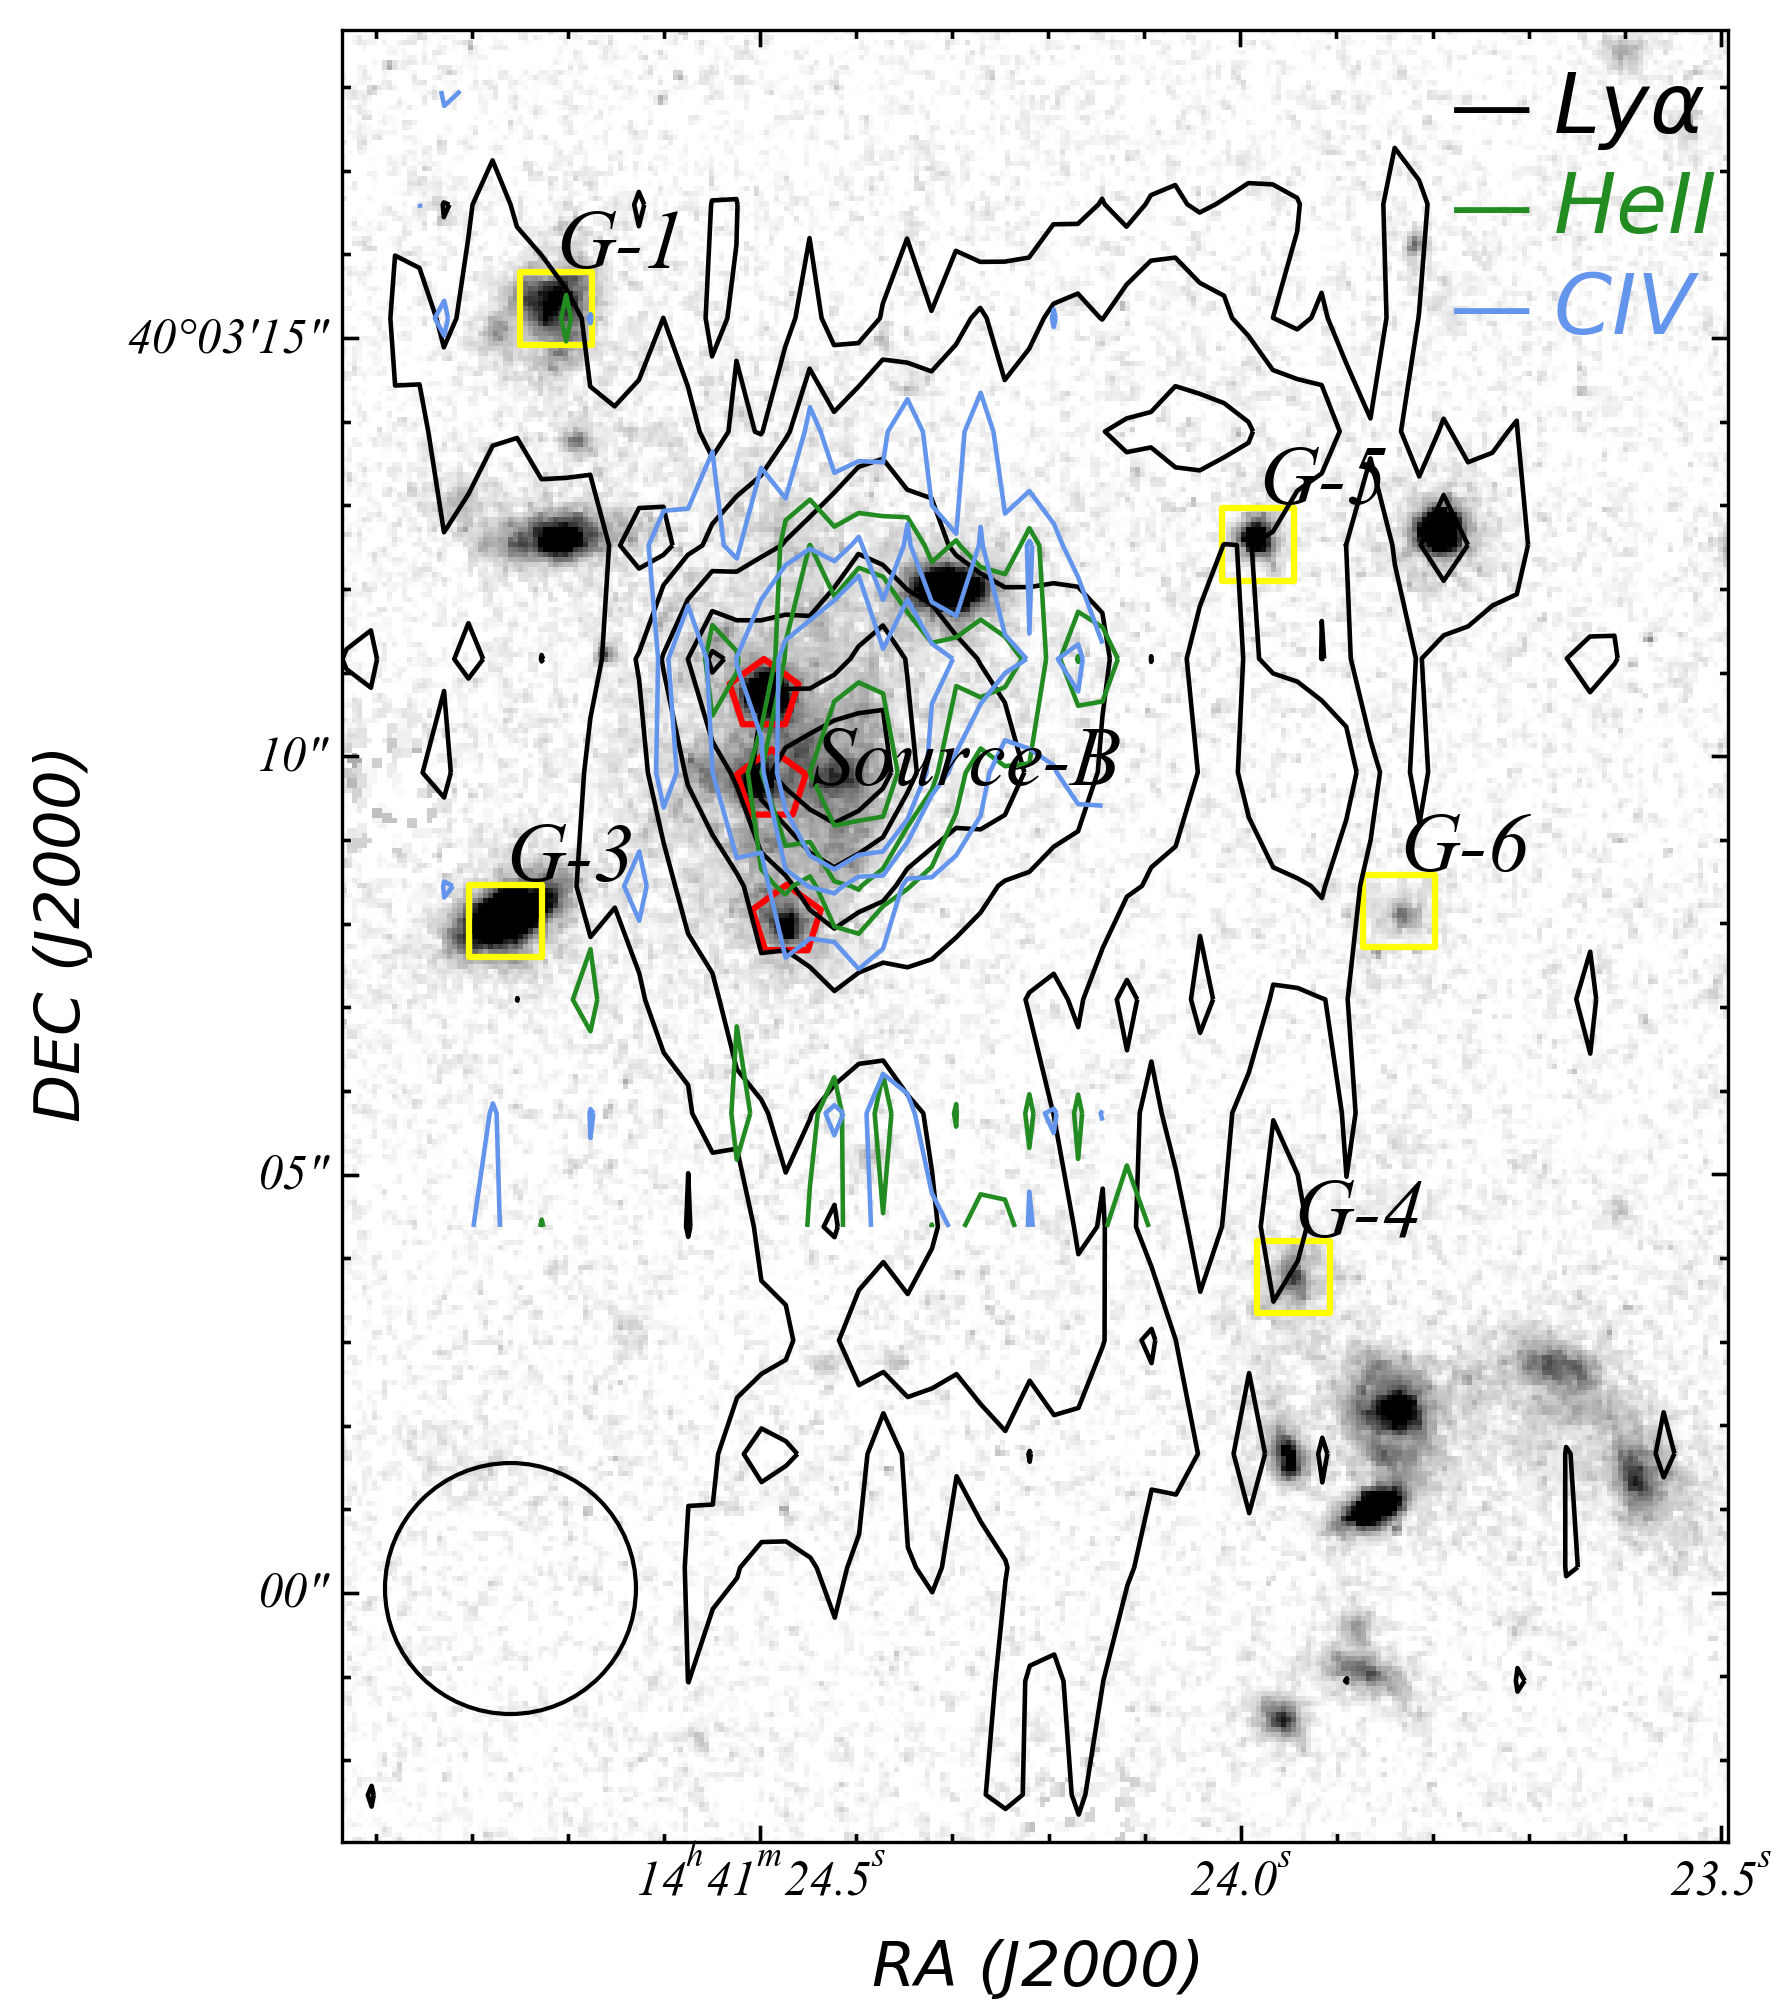
\includegraphics[width=0.5\textwidth]{figs/contour}}
		\subfloat[spectra]{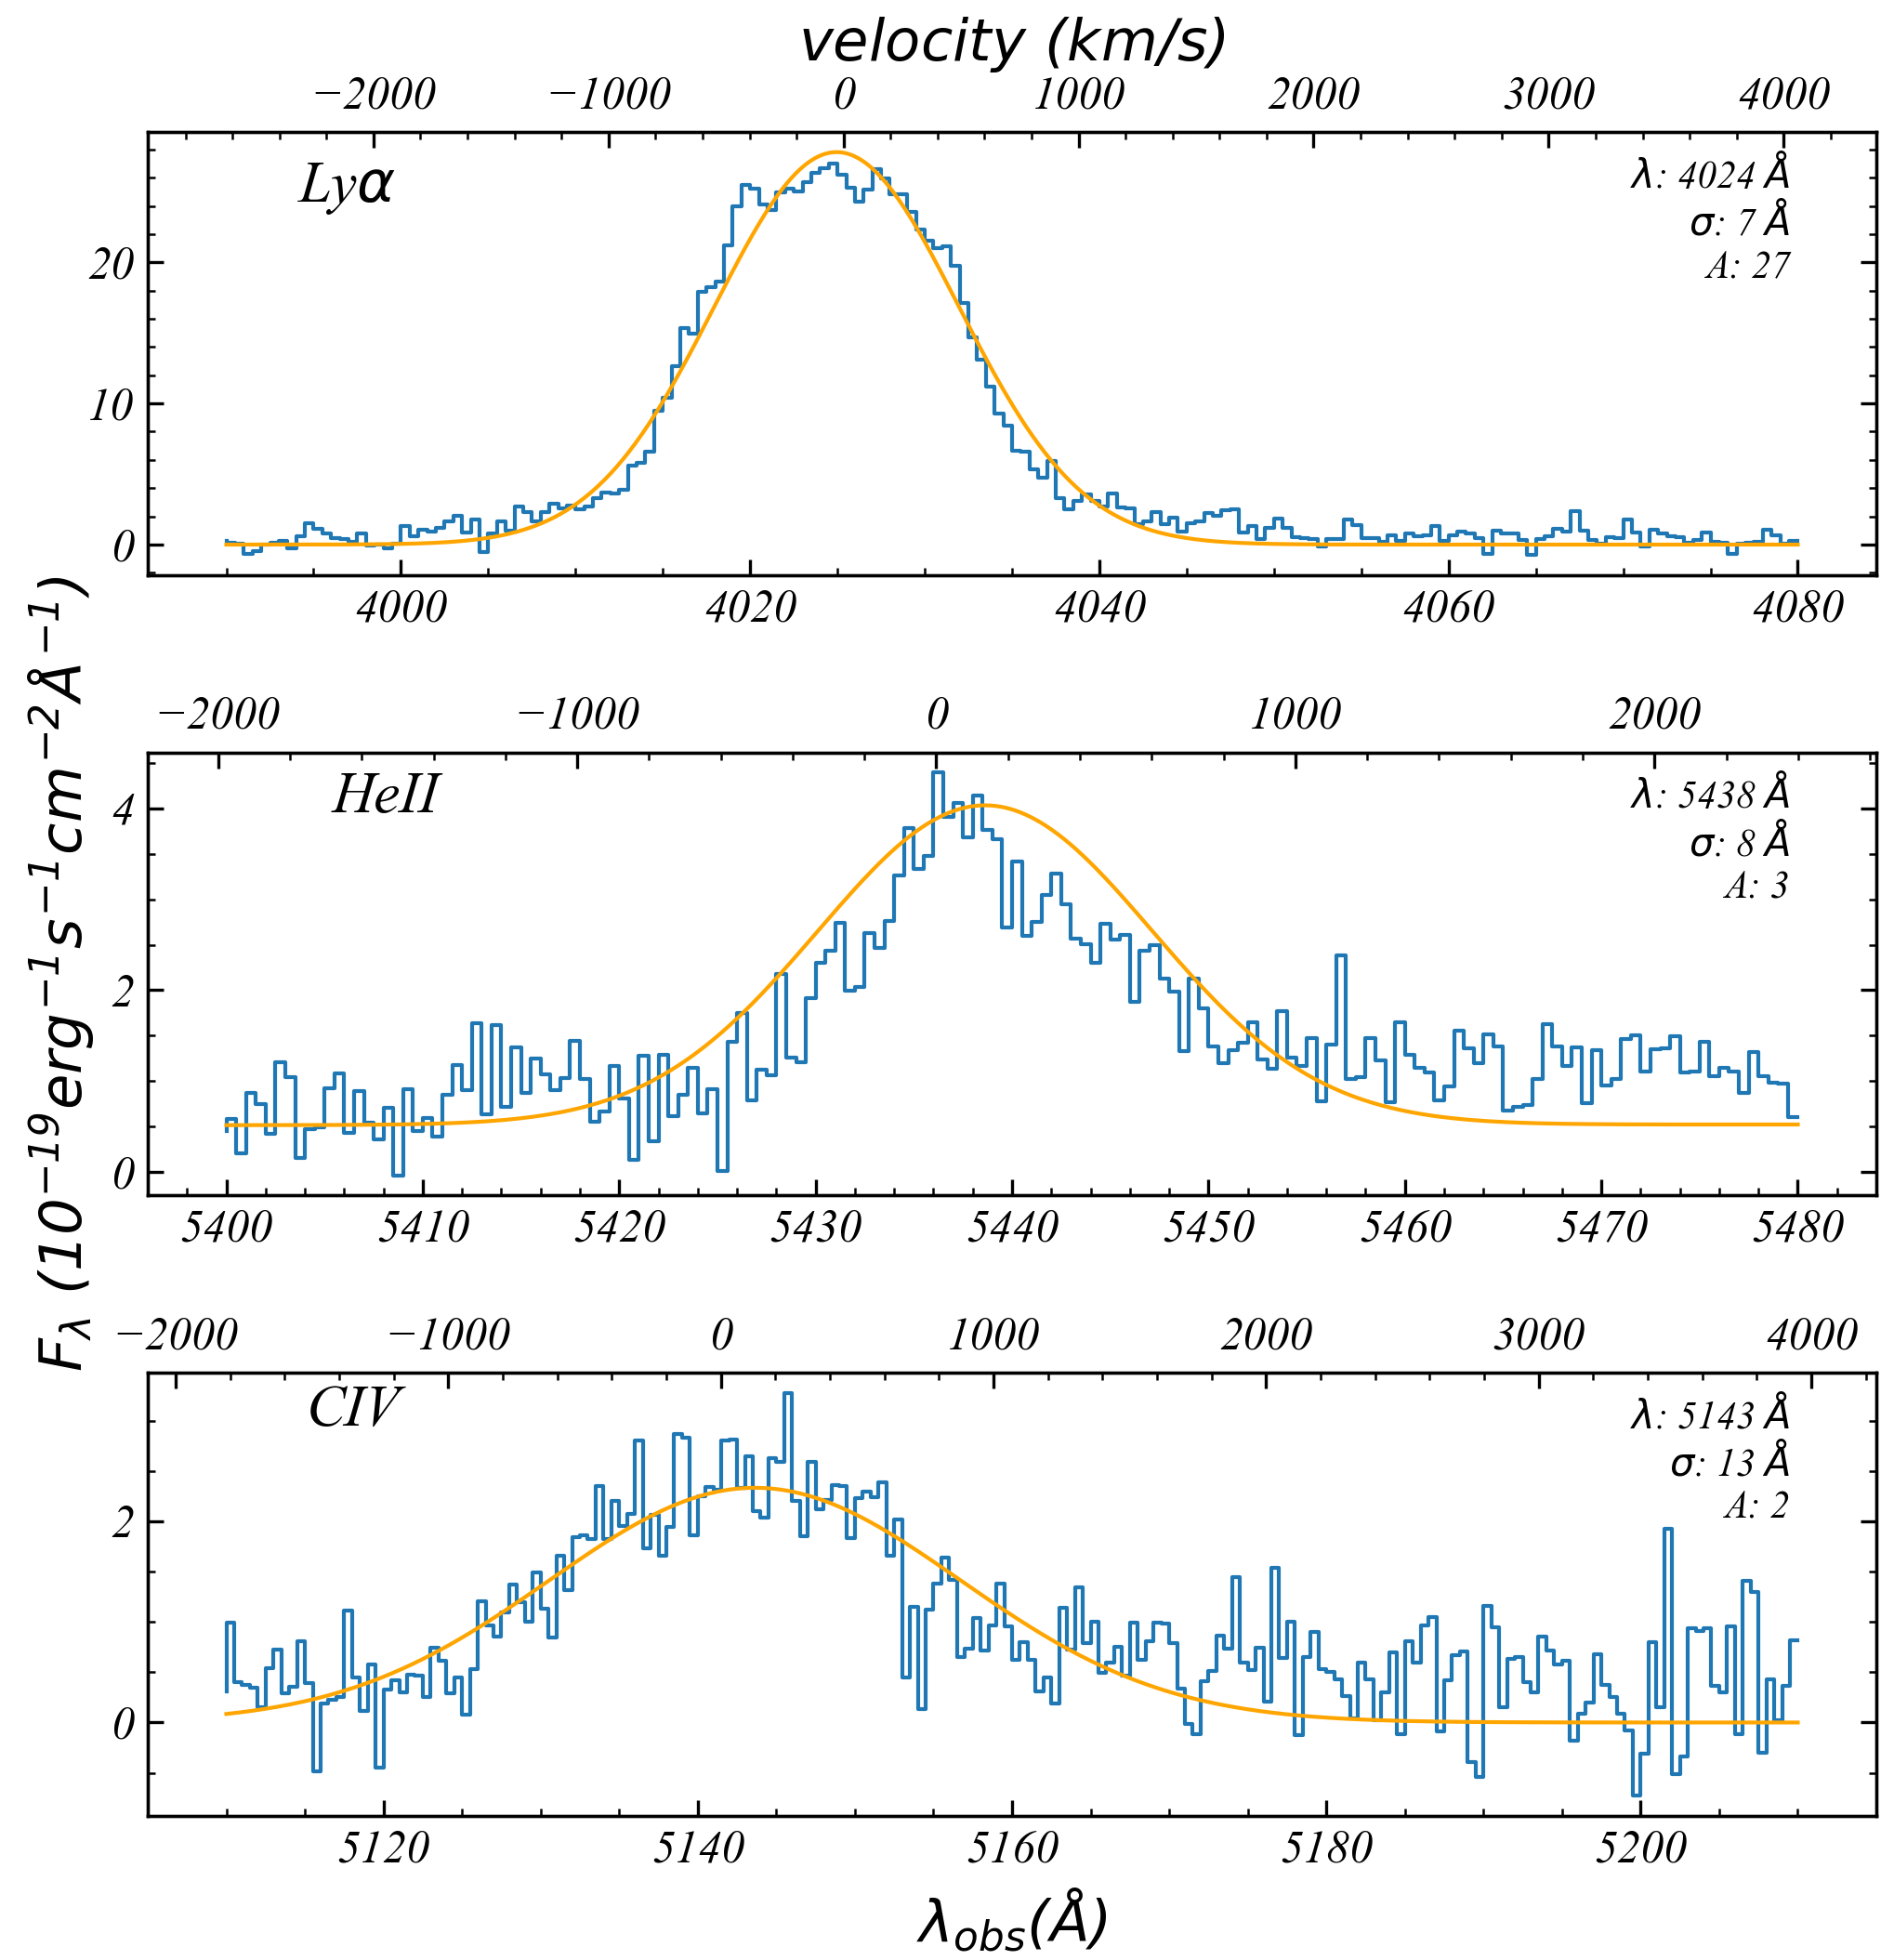
\includegraphics[width=0.5\textwidth]{figs/spectral}}
		\label{overlayspec}
		\caption{Left: HST image of MAMMOTH-1 from circle 24,25, PI: Cai. We overlay on it ly$\alpha$ HeII and CIV psudo narrow band images. Black contour is ly$\alpha$, blue contour is HeII, green contour is CIV. We also mark source-B with red mark and sources at the same redshift with yellow mark. We also plot circle with raidus of 1$arcsec^{2}$. Right: spectra of the 3 emission lines extracted from aperture center on source-B with radius 1$arcsec^{2}$, we fit them with one-component gaussian function.}
	\end{figure*}
	\begin{table}[htp]
	\begin{center}
		\begin{tabular}{ccccc}
\hline
\hline
& $\lambda_{c}(A)$ & $\sigma_{\lambda}(A)$ & L(erg/s) & redshift \\ \hline
ly$\alpha$ &   4024  &     7  &   $2.68 \times 10^{44}$ & 2.310        \\
HeII       &   5438  &     8  &   $1.97 \times 10^{43}$ & 2.316        \\
CIV        &   5143  &     13 &   $2.29 \times 10^{43}$ & 2.320        \\ \hline
\end{tabular}
\end{center}
	\caption{}
	\label{fit_L}
	\end{table}

\end{document}